\documentclass[a4paper]{article}
\usepackage[UTF8]{ctex}
\usepackage{geometry}
\usepackage{graphicx}
\usepackage{url}
\usepackage{multirow}
\usepackage{array}
\usepackage{booktabs}
\usepackage{url}
\usepackage{enumitem}
\usepackage{graphicx}
\usepackage{float}
\usepackage{amssymb}
\usepackage{amsmath}
\usepackage{subfig}
\usepackage{longtable}

\geometry{a4paper, scale=0.78}

\title{Exponential Family Distribution 01}
\author{Chen Gong}
\date{22 October 2019}

\begin{document}

\maketitle

本节主要对指数族分布的概念和性质的一个小小的总结。指数族分布是一个广泛存在于机器学习研究中的分布。包括,Guassian分布,Bernoulli分布(类别分布),二项分布(多项式分布),泊松分布,Beta分布,Dirichlet分布,Gamma分布和Gibbs分布等。

\section{指数族分布的基本形式}
指数族分布的基本形式可以表示为:
\begin{equation}
    p(x|y)=h(x)exp\left\{ \eta^T\varphi(x)-A(\eta) \right\}
\end{equation}

$\eta$:参数向量,$\eta \in \mathbb{R}^p$。

$A(\eta)$:log partition function (配分函数)。

$h(x)$:这个函数只和$x$有关系,所以并不是很重要。

$\eta$和$h(x)$的理解比较简单,但是log partition function的理解难度比较大。所以,在这里对此函数做出一定的解释。

\subsection{log partition function (配分函数)}
什么是配分函数呢?我的理解这是一个归一化的函数因子,用来使概率密度函数的积分值为1。推导过程如下:
\begin{equation}
    \begin{split}
        p(x|\theta) =  & \frac{\hat{p}(x|\theta)}{z} \\
        \int p(x|\theta) dx = & \int \frac{\hat{p}(x|\theta)}{z}dx = 1 \\
        z = & \int \hat{p}(x|\theta)dx
    \end{split}
\end{equation}

而在指数族函数中有关于$A(\eta)$的配分函数的推导如下:

\begin{equation}
    \begin{split}
        p(x|\eta) = & h(x)exp\{ \eta^T\varphi(x)\}exp\{-A(\eta)\} \\
        = & \frac{1}{exp\{A(\eta)\}} h(x)exp\{ \eta^T\varphi(x)\}\\
        \int p(x|\eta) dx = & \int \frac{1}{exp\{A(\eta)\}} h(x)exp\{ \eta^T\varphi(x)\} dx = 1 \\ 
        exp\{A(\eta)\} = & \int h(x)exp\{ \eta^T\varphi(x)\} dx \\ 
        A(\eta) = & \log \int h(x)exp\{ \eta^T\varphi(x)\} dx
    \end{split}
\end{equation}

所以,$A(\eta)$被称为带有的log的Partition Function。 

\section{指数族分布的相关知识}
和指数族分布的相关知识,可以用下面这张图表来进行概况。
\begin{figure}[H]
    \centering
    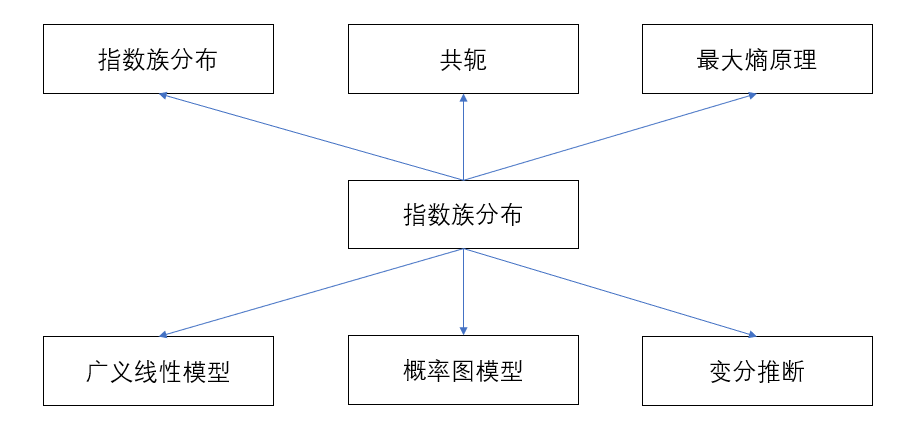
\includegraphics[width=.8\textwidth]{微信图片_20191022170308.png}
    \caption{指数族分布相关知识表示图}
    \label{fig:my_label_1}
\end{figure}

\subsection{充分统计量}
什么是充分统计量?我自己的理解,充分统计量是一个有关于样本的函数,有了这个统计量就可以完整的表示出数据集整体的特征。从某种意义上说,我们就可以丢弃样本数据集了。下面对Guassian Distribution进行举例,数据集Data set为:$\{x_1,x_2,x_3,\cdots ,x_N\}$

我们只需要一组充分统计量:
\begin{equation}
    \varphi(x) = 
    \begin{pmatrix}
        \sum_{i=1}^Nx_i \\
        \sum_{i=1}^Nx_i^2
    \end{pmatrix}
\end{equation}
就可以反映出Guassian的所有特征$\theta=(\mu, \Sigma)$。充分统计量在online learning中的使用有很大的作用。这样可以不记录那么多的数据集,只使用少量的数据就可以估计得到数据集整体的特征,可以用来简化计算。

\subsection{共轭}
为什么要使用共轭的概念呢?首先来看看贝叶斯公式:
\begin{equation}
    p(z|x)=\frac{p(x|z)p(z)}{\int_{z}p(x|z)p(z)dz}
\end{equation}

在这个公式中,$p(z|x)$为后验概率分布,$p(x|z)$为似然函数,$p(z)$为先验分布。在求解$\int_{z}p(x|z)p(z)dz$时,计算难度是非常大的。或者说很多时候,根本算不出来。而且,换句话说,就算我们求得了$p(z|x)$,也有可能因为$p(z|x)$的形式过于复杂,导致$\mathbb{E}_{p(z|x)}[f(x)]$根本算不出来。所以,为了解决这个问题,科研人员们想了很多的办法。近似推断的方法,比如,变分和采样。

变分的方法,是用简单的分布来拟合一个很难计算的分布,从而计算得出$p(z|x)$的近似分布形式。而采样的方法,比如蒙特卡罗采样,隐马尔可夫蒙特卡罗采样(MCMC)等,是直接来求$\mathbb{E}_{p(z|x)}[f(x)]$,这样直接跳过了中间那一堆的过程,在强化学习中经常使用。

而共轭是一种很取巧的方法,它的效果是使先验和后验有着相同的分布形式。这样可以大大的简化计算,解决上述的问题。举例,
\begin{equation}
    p(z|x)\varpropto p(x|z)p(z)
\end{equation}

如果,$p(x|z)$为二项分布,$p(z)$为Beta分布,那么后验分布$p(z|x)$也为Beta分布。

\subsection{最大熵原理}
下面列举几种确定先验(prior distribution)的方法,
\begin{enumerate}[itemindent = 1em, itemsep = 0.4pt, parsep=0.5pt, topsep = 0.5pt]
\item 共轭,主要是为了计算的简单;
\item 最大熵方法,主要是为了解决无信息先验问题;
\item Jerrif。
\end{enumerate}

最大熵原理会在后面的小节做详细的描述,主要思想就是“等可能”。也就是尽量使所有的结论等可能的出现,来增加不确定性,保证每一项都是公平的。

\subsection{广义线性模型}
广义线性模型包括:
\begin{enumerate}[itemindent = 1em, itemsep = 0.4pt, parsep=0.5pt, topsep = 0.5pt]
\item 线性组合,比如,$w^Tx$;
\item link function,也就是激活函数的反函数;
\item 指数族分布,$y|x\sim$指数族分布,包括:
    \begin{enumerate}[itemindent = 1em, itemsep = 0.4pt, parsep=0.5pt, topsep = 0.5pt]
        \item 线性回归,在我们的线性回归模型中,我们曾定义过假设噪声符合Guassian Distribution,那么$y|x\sim\mathcal{N}(\mu, \Sigma)$;
        \item 二分类问题:
        \begin{enumerate}[itemindent = 1em, itemsep = 0.4pt, parsep=0.5pt, topsep = 0.5pt]
            \item $y|x\sim$Bernoulli分布;
            \item $y|x\sim$Possion分布;
        \end{enumerate}
    \end{enumerate}
\end{enumerate}

\subsection{概率图模型和变分推断}
包括无向图等,有玻尔兹曼滤波器等。后续的章节会进行详细的描述。变分推断也在后续的章节有详细的描述。

\end{document}
